%% ---------------------------
% Zusätzliche Pakete und Definitionen
%% ---------------------------

\usepackage[utf8]{inputenc}
\usepackage[english]{babel} % Sprachanpassungen und Trennmuster
\usepackage[T1]{fontenc}    % T1 Schrift Encoding
\usepackage{textcomp}       % zusätzliche Symbole (Text Companion)
\usepackage{mathptmx}              %% --- Times mit Matheschriften
% \usepackage{mathpazo}            %% --- Palatino
\usepackage[scaled=.90]{helvet}    %% --- Helvetica

%\usepackage{fontspec} % Font selection for XeLaTeX; see fontspec.pdf for
% documentation
%\defaultfontfeatures{Mapping=tex-text} % to support TeX conventions like
% ``---''
%\usepackage{xunicode} % Unicode support for LaTeX character names (accents,
% European chars, etc)
%\usepackage{xltxtra} % Extra customizations for XeLaTeX

%\setmainfont{Myriad Pro} % set the main body font (\textrm), assumes Charis SIL
% is installed
%\setsansfont{Myriad Pro}

\usepackage{booktabs}
\usepackage{multimedia}
\usepackage{listings}

\usepackage[acronym,nomain]{glossaries}
\newcommand*{\glossfirstformat}[1]{\color{red}\textbf{#1}}
\renewcommand{\glsdisplayfirst}[4]{\glossfirstformat{#1#4}}
\renewcommand*{\glsnamefont}{\sffamily}


\usepackage{color}

\definecolor{pblue}{rgb}{0.13,0.13,1}
\definecolor{pgreen}{rgb}{0,0.5,0}
\definecolor{pred}{rgb}{0.9,0,0}
\definecolor{pgrey}{rgb}{0.46,0.45,0.48}

\lstset{language=Java,
  showspaces=false,
  showtabs=false,
  breaklines=true,
  showstringspaces=false,
  breakatwhitespace=true,
  commentstyle=\color{pgreen},
  keywordstyle=\color{pblue},
  stringstyle=\color{pred},
  basicstyle=\ttfamily\scriptsize,
  moredelim=[il][\textcolor{pgrey}]{$$},
  moredelim=[is][\textcolor{pgrey}]{\%\%}{\%\%}
}

\usepackage{enumerate}

\graphicspath{{RT01-Introduction/}{01principles/}{02swarchitectures/}}
%% ---------------------------
% Beamer Theme
%% ---------------------------
\usetheme{Esslingen}

%\usecolortheme{default}  %      kein Farb-Hintergrund in Blöcken
%\usecolortheme{lily}     %      kein Farb-Hintergrund in Blöcken
 \usecolortheme{rose}     %  dezenter Farb-Hintergrund in Blöcken
%\usecolortheme{orchid}   % kräftiger Farb-Hintergrund in Blöcken

\setbeamercovered{transparent=30}

%% ---------------------------
%% Definitionen für die Titelseite
%% ---------------------------
%% Die optionalen Argumente werden für die Fußzeile benutzt

\ifoverview
\title[Distributed Real Time Systems - \partTitle \ (Version \partVersion)]{Distributed Real Time Systems}

\subtitle[\partTitle]{\partTitle}

\else

\title[Distributed Real Time Systems - Part \partNo :\ \partTitle \ (Version \partVersion)]{Distributed Real Time Systems}

\subtitle[Part  \partNo :\  \partTitle]{Part \partNo : \  \partTitle}

\fi

\author[Vikas Agrawal]{Vikas Agrawal}% \and
 %Zweiter Autor\inst{1} \and
 %Dritter Autor\inst{2}}

%% Default image
\titlegraphic{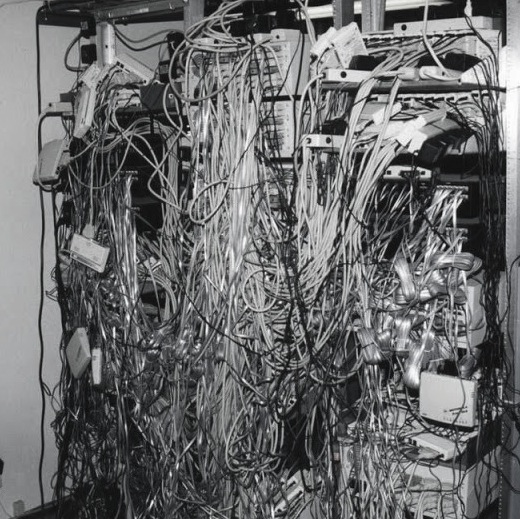
\includegraphics[height=125pt]{RT00-Introduction/dtrt.png}}

\ifpartII
\titlegraphic{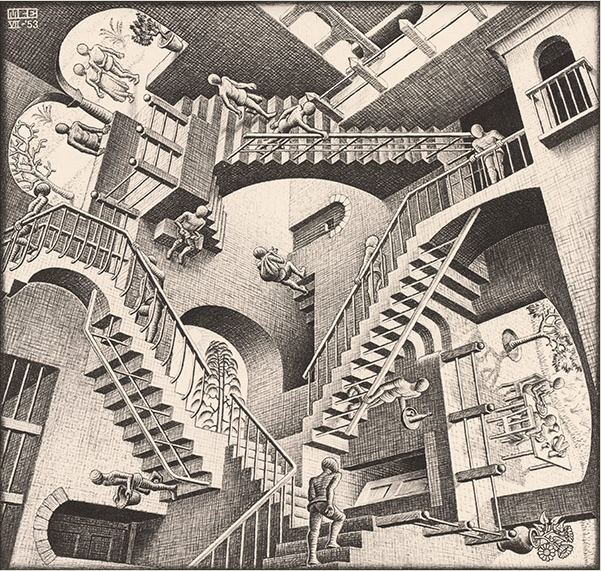
\includegraphics[height=125pt]{02swarchitectures/escher2.png}}
\fi

\institute[University of Applied Sciences Esslingen]{%
%\inst{1}University of Applied Sciences Esslingen, Faculty of Information Technology
%  \and
% \inst{2}Andere Einrichtung
}

\date[\copyright{} 2015]{\today}

%\makenoidxglossaries

%% ---------------------------
% Glossary
%% ---------------------------

\newglossaryentry{umll}{name={Unified Modelling Language},
 description={Unified Modelling Language}}

\newglossaryentry{UML}{name={UML},
 description={Unified Modelling Language}}


\newglossaryentry{model}{name={model},plural={models},
 description={model}}


\newglossaryentry{structure}{name={structure},
 description={structure}}

\newglossaryentry{behaviour}{name={behaviour},
 description={behaviour of something}}

\newglossaryentry{attribute}{name={attribute}, description={describe the appearance and knowledge of a class of objects}}
\newglossaryentry{operation}{name={operation}, description={define the behavior that a class of objects can manifest}}
\newglossaryentry{stereotype}{name={stereotype}, description={ help you understand this type of object in the context of other classes 
                of objects with similar roles within the system’s design}}
\newglossaryentry{property}{name={property}, plural={properties}, description={ provide a way to track the maintenance and status of the class definition}}
\newglossaryentry{association}{name={association}, description={ is just a formal term for a type of relationship that this type of object may participate in. 
                 Associations may come in many variations, including simple, aggregate and composite, qualified, and reflexive.}}
\newglossaryentry{inheritance}{name={inheritance}, description={ allows you to organize the class definitions to simplify and facilitate their implementation.}}



